A respeito do fatores comentados na seção anterior, \citeonline{bhalerao09} concluem que são oito os fatores vitais que afetam o 
custo, tamanho e duração (CTD) em métodos de estimativa ágeis. Estes são descritos a seguir:

\subsection{Project Domain (Domínio do Projeto)}
  
  Existem diferentes atividades envolvidas para diferentes domínios de projeto \cite{jones07}. Cada domínio é caracterizado por
  diferentes tipos e número de atividades, o que afeta de forma peculiar o CTD. Portanto, o domínio do projeto deve ser levando em consideração para
  se realizar uma estimativa.

\subsection{Performance (Desempenho)}
 
  O fator desempenho em um projeto pode ser caracterizado como tempo de execução, \textit{design} e padrões de codificação, precisão
  no resultado, entre outros. Geralmente, questões de desempenho são descritas pelos requisitos não-funcionais do software \cite{bhalerao09}.
  Portanto, para se atingir os níveis de desempenho exigidos pelo cliente, é necessário incluir recursos no projeto e na arquitetura
  do software, o que, dependendo do recurso, pode aumentar o custo e duração do projeto \cite{bhalerao09}.
  
\subsection{Configuration (Configuração)}
 
  O fator configuração refere-se a requisitos especiais de hardware e software necessários para executar o software sem problemas.
  Para \citeonline{bhalerao09} é um dos fatores chave na estimativa do CTD, pois projetos que necessitam de configurações especiais
  certamente aumentam o custo e os esforços no projeto, codificação e implementação do software.
  
\subsection{Data Transaction (Transação de Dados)}
 
 O fator transação de dados refere-se ao volume e frenquência da transferência de dados no software \cite{bhalerao09}. Quando o volume
 de transação de dados é alto, o \textit{design} e desenvolvimento são afetados, o que exige maior esforço para desenvolver o software
 e, portanto, aumenta o seu custo \cite{bhalerao09}.
   
\subsection{Complex Processing (Processamento complexo)}
 
 Um projeto de software pode exigir um processamento complexo dos dados \cite{bhalerao09}. Regras científicas ou regras comerciais, acesso
 remoto de computadores, entre outros podem aumentar o fator de complexidade de processamento, o que requer atenção especial em vários estágios 
 do desenvolvimento, resultando no aumento de custo e duração do projeto \cite{bhalerao09}.
 
\subsection{Ease of Operation (Facilidade de operação)}
 
 O fator de facilidade de operação pode ser conceituado como sendo o forncimento de facilidades ao usuário na operação do sistema \cite{bhalerao09}.
 Porém, o projeto e arquitetura do software devem incluir os recursos necessários para proporcionar maior facilidade de utilização ao
 usuário, o que aumenta o CTD do projeto \cite{bhalerao09}.
 
\subsection{Multiple Sites (Múltiplos Sites)}

 Se o software roda em vários sites ou muitos membros do time trabalham juntos em ambinetes distribuidos, o custo do projeto irá aumentar
 devido às complexidades de comunicação e coordenação da equipe. Portanto, este deve ser um fator que deve-se considerar na estimativa
 de duração do projeto \cite{bhalerao09}.
 
\subsection{Security (Segurança)}

 O fator segurança refere-se à segurança dos dados, segurança operacional, segurança de código, entre outros \cite{bhalerao09}. Todos estes
 aspectos de segurança devem ser pensados no momento da concepção, codificação e implementação, o que aumenta a complexidade do projeto
 e, consequentemente, o CTD do projeto como um todo \cite{bhalerao09}.
 
\subsection{Classificação dos fatores}

A técnica proposta por \citeonline{bhalerao09} prevê que os fatores sejam classificados em três níveis de intensidade, como explicado na seção \ref{algoritmo}.
São eles: \textit{Low, Medium} e \textit{High}.
Para a classificação dos fatores nos diferentes níveis, deve-se atentar a Figura \ref{cla_fatores} a seguir:

  \begin{figure}[!htb]
    \centering
    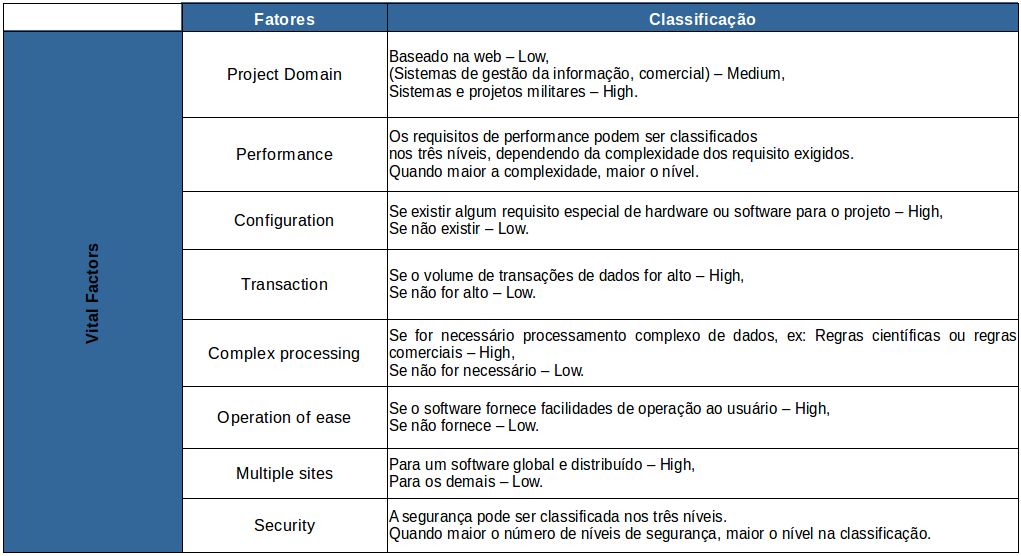
\includegraphics[scale=0.40]{figuras/fatores}
    \caption{Classificação dos fatores. Adaptada de: \cite{bhalerao09}.}
    \label{cla_fatores}
  \end{figure}